\documentclass{oblivoir}

\usepackage{amsthm}
\usepackage{thmtools}

\usepackage{url}

%\usepackage{ansform}
\usepackage{ikps}

\usepackage{graphicx}
%https://www.overleaf.com/learn/latex/Inserting_Images

\usepackage{listings}
\usepackage{xcolor}
\declaretheoremstyle[% spaceabove=6pt,spacebelow=6pt, headfont=\color{MainColorOne}\sffamily\bfseries, notefont=\mdseries, notebraces={[}{]}, bodyfont=\normalfont,
headpunct={},
postheadspace=1em,
%qed=▣,
]{maintheorem}

\declaretheorem[%
name=정의,
style=maintheorem,
numberwithin=section, shaded={%bgcolor=MainColorThree!20,
margin=.5em}]{dfn}
% \begin{dfn}[]
% \end{dfn}

\newtheorem{theorem}{Theorem}[section]
\newtheorem{corollary}{Corollary}[theorem]
\newtheorem{lemma}[theorem]{Lemma}
%https://www.overleaf.com/learn/latex/Theorems_and_proofs

\definecolor{mGreen}{rgb}{0,0.6,0}
\definecolor{mGray}{rgb}{0.5,0.5,0.5}
\definecolor{mPurple}{rgb}{0.58,0,0.82}
\definecolor{backgroundColour}{rgb}{0.95,0.95,0.92}
%https://tex.stackexchange.com/questions/348651/c-code-to-add-in-the-document
\lstdefinestyle{CStyle}{
    backgroundcolor=\color{backgroundColour},   
    commentstyle=\color{mGreen},
    keywordstyle=\color{magenta},
    numberstyle=\tiny\color{mGray},
    stringstyle=\color{mPurple},
    basicstyle=\footnotesize,
    breakatwhitespace=false,         
    breaklines=true,                 
    captionpos=b,                    
    keepspaces=true,                 
    numbers=left,                    
    numbersep=5pt,                  
    showspaces=false,                
    showstringspaces=false,
    showtabs=false,                  
    tabsize=2,
    language=C
}

\title{All about Quick Sort}
\author{이윤승}

\begin{document}
    

\maketitle


\tableofcontents

\section{소개}

\begin{itemize}
    \item 일반적으로 가장 많이 사용하는 정렬 알고리즘
    \item 비교 정렬
    \item 내부정렬
    \item 불안정 정렬
    \item 평균 복잡도: $O(n \lg n)$
    \item 최악의 복잡도 : $O(n^2)$
    \item C++ std::sort의 내부구현이 퀵소트로 되어있음
\end{itemize}

\section{의사코드 및 동작}

분할 정복(divide and conquer) 방법을 통해 설계 되었다.
당장에 유튜브에 검색만해봐도 동작 설명하는 5분짜리 유튜브가 많으니 그걸 참고하는게 편하다.

\begin{lstlisting}[style = CStyle]    
QUICKSORT(A,p,r)
    if p < r
        q = PARTITION(A,p,r)
        QUICKSORT(A,p,q-1)
        QUICKSORT(A,q+1,r)
\end{lstlisting}

\begin{lstlisting}[style = CStyle]
PARTITION(A ,p ,r)
    x= A[r] //pivot
    i = p-1
    for j = p to r-1
        if A[j]<= x
            i = i + 1
            exchange A[i] with A[j]
    exchange A[i+1] with A[r]
    return i + 1
    
\end{lstlisting}

PARTITION 프로시저의 시간복잡도는 $\Theta(n)$이다.

\url{https://www.youtube.com/watch?v=hq4dpyuX4Uw&list=PL52K_8WQO5oUuH06MLOrah4h05TZ4n38l&index=11}

\begin{figure}[h!]
    \centering
    \includegraphics[scale=0.7]{{q1.png}}
    \caption{quick sort 작동 예시}
\end{figure}



성능 참고 : 
\url{https://www.acmicpc.net/blog/view/58}



\section{복잡도 분석}

\subsection{최악의 분할 케이스} 

최악의 경우 분할 케이스를 생각해보자 
이는 왼쪽 오른쪽 분할이 한쪽으로 쏠려(오름차순,내림차순) 극도로 불균형하게 일어났을때이다.
피봇값에 의한 분할이 아예 일어나지 않을 때 최악의 케이스가 된다.
이때 비용을 나타낸 재귀함수다.
$$T(n) = T(n-1) + cn $$

\begin{align*}
    T(n) &= T(n-1) + cn \\
    &= T(n-2) + c(n-1) +cn \\
    &= c\sum^{n}_{k=1}k \\
    &= \dfrac{1}{2} cn^{2}\\
    &= \Theta (n^{2})    
\end{align*}


따라서 시간복잡도는 $\Theta(n^2)$이다.

\subsection{최선의 분할 케이스} 

정확하게 반으로 나누어 졌을때 최선의 분할 케이스이다.

이때의 비용을 나타낸 재귀함수는
$$T(n) = 2T(n/2) + cn$$
이다.

\begin{figure}[h!]
    \centering
    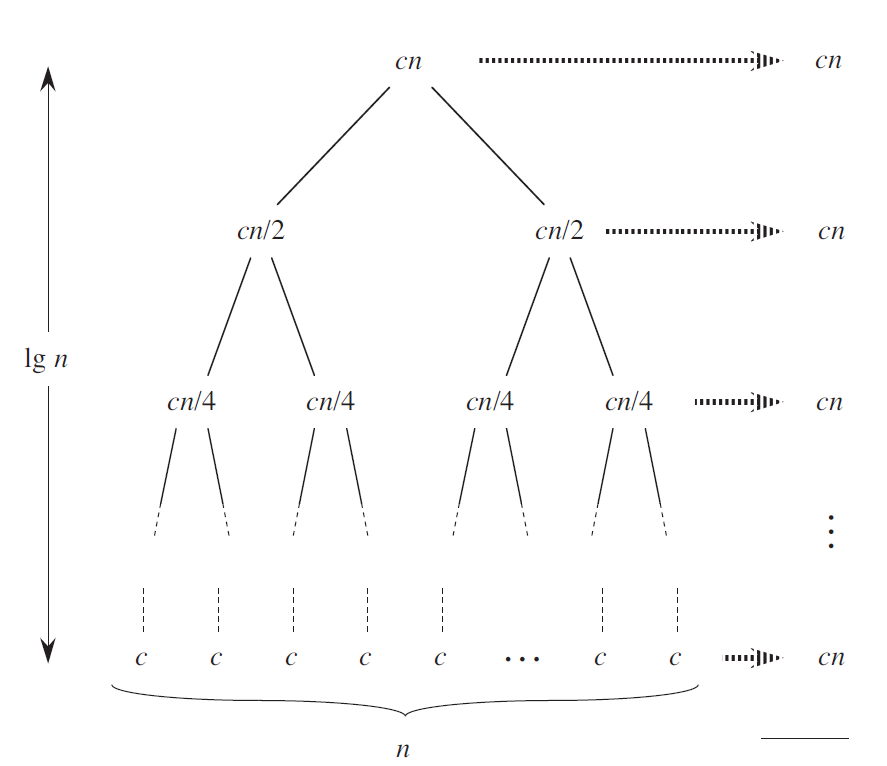
\includegraphics[scale=0.5]{q2.png}
    \caption{quick sort 최선의 분할 케이스 재귀 트리}
\end{figure}
그림 2의 재귀트리를 통해서 전체 비용을 계산하여 시간복잡도를 구하면 $\Theta(n \lg n)$이다.

\subsection{직관적인 일반적인 케이스 방법} 

랜덤한 분할의 퀵소트를 가정하기 위해서 최선의 분할 케이스와 최악의 분할 케이스가 번갈아 나타난다고 생각해보자

\begin{figure}[h!]
    \centering
    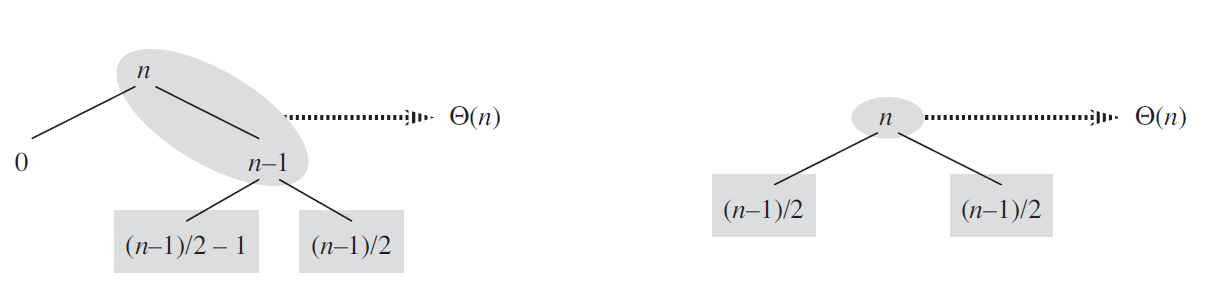
\includegraphics[scale=0.5]{q3.png}
    \caption{quick sort 일반적인 재귀 트리}
\end{figure}

T(n) 일때의 시간복잡도와 T(n-1)일때의 시간복잡도는 둘다 $\Theta(n)$이다. 따라서 이 둘의 시간복잡도를 합쳐도 결국 $\Theta(n)$이고 이를 합쳐서 보면 결국에 최선의 분할 케이스가 된다 따라서 이때의 시간복잡도는 결국 $\Theta(n \lg n)$이다.

\section{상세 분석}

\subsection{최악의-케이스 분석 }


실제 재귀함수를 일반화 식은 다음이 된다.

$$T(n) = \max_{0 \le q \le n-1}(T(q) + T(n-q-1)) + \Theta(n)$$

이때 $T(n)$이 $\Theta(n^2)$임을 보이면된다.
치환법을 이용해서 이 점화식을 풀수있다.
$T(n) \le c_1n^2$이라 가정하자. 그러면

$$T(n) \le \max_{0 \le q \le n-1}(c_1q^2 + c_1(n-q-1)^2) + \Theta(n)$$

이 성립한다. 

$0 \le q \le n-1$인 $c_1q^2 + c_1(n-q-1)^2$에 대해서 

$f(q) = c_1q^2 + c_1(n-q-1)^2$ 이라하고 $f'(q) = 2c_1q - 2c_1(n-q-1)$이므로 $q=\dfrac{n-1}{2}$일때 극솟값을 가진다. 이 극솟값은 $q$의 존재 범위에 포함되고 따라서 이차함수의 특성에 따라 양 끝점이 최댓값이 될수있는 후보가된다. $q=0$일때와 $q=n-1$일때 극댓값을 가지는데 이때의 두 함숫값은 같아서 둘중 어느값을 택해도 최댓값이 된다.

\begin{align*}
    T(n) & \le c_1(n-1)^2 + \Theta(n) \\
    & \le c_1n^2 - c(2n-1) + \Theta(n) \\
    & \le c_1n^2    
\end{align*}


이때 $\Theta(n) = dn$에서 $ c_1 > d $인 상수 $c_1$을 가지게 함으로 써 결과적으로 $T(n)$이 $c_1n^2$보다 작거나 같음을 보일수있다. 반대로 $c_2n^2 \le T(n)$임을 가정하고  $ c_2 < d $인 상수를 잡음으로 $T(n)$이 $c_2n^2$보다 크거나 같음을 보일수있다. 따라서 $T(n) = \Theta(n^2)$를 얻을 수 있다.



\section{여러 기초 지식}

\subsection{시간복잡도}

\begin{dfn}[복잡도]
    상한, 하한,  
    \begin{itemize}

        \item 상한 big O
        
        함수 $f(n), g(n)$에 대해서 $0 \le f(n) \le cg(n) ( \forall n \leq n_0)$을 만족하는 $n_0$, 양의 상수 $c$가 존재할때 $f(n) = O(g(n))$이라한다.
        
        \item 하한 omega

        함수 $f(n), g(n)$에 대해서 $0 \le cg(n) \le f(n) ( \forall n \leq n_0)$을 만족하는 $n_0$, 양의 상수 $c$가 존재할때 $f(n) = \Omega(g(n))$이라한다.

        \item Theta

        $\Theta(g(n))$일 필요충분 조건은 $f(n) = O(g(n))$이고 $f(n) = \Omega(g(n))$이 성립할때 이다.
    \end{itemize}
\end{dfn}

\subsection{조화 급수의 상한과 하한}



$\sum_{k=1}^{n} \dfrac{1}{k} = \Theta(\lg n)$

감소 함수 $f(k)$에 대해서 다음이 성립한다

$$\int_{m-1}^{n}f(x)dx \le \sum_{k=m}^n f(k) \le \int_{m}^{n+1}f(x)dx$$


\begin{figure}[h!]
    \centering
    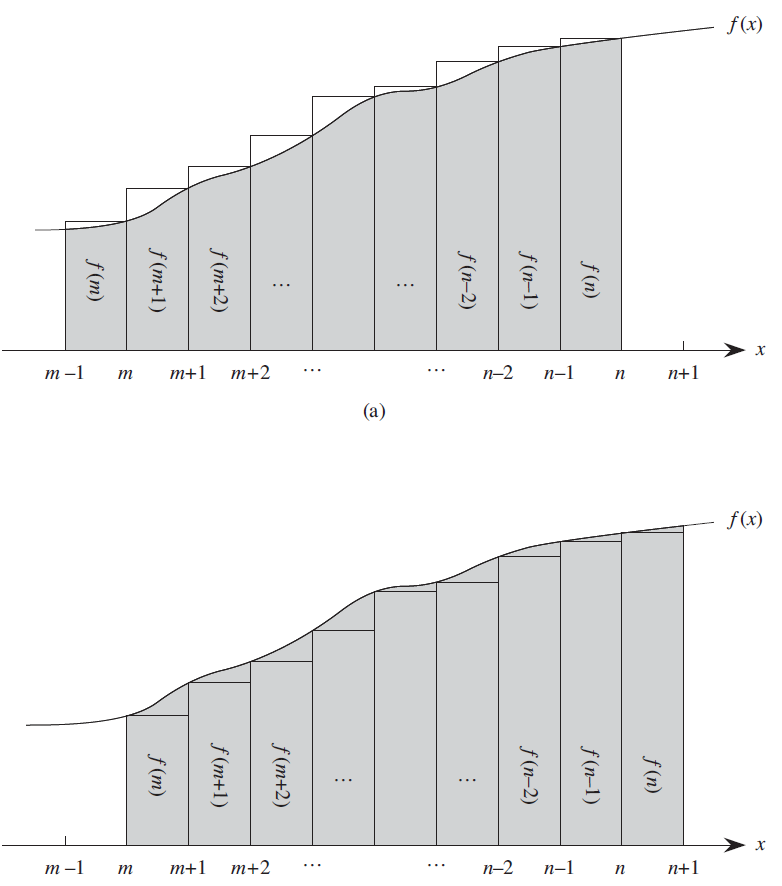
\includegraphics[scale=0.5]{q5.png}
    \caption{증가함수의 대소비교}
\end{figure}

증가함수 $f(k)$에 대해 다음이 성립함을 그림 4를 통해서 이해 할 수있다. 감소함수는 이와 반대로 생각하면 쉽게 해당 부등식을 이해할 수 있다.

$$\int_{m}^{n+1}f(x)dx \le \sum_{k=m}^n f(k) \le \int_{m-1}^{n}f(x)dx$$

다음 두가지 방식으로 계산한다

$\sum_{k=2}^n \dfrac{1}{k}+1 \le \int_{2}^{n+1}f(x)dx +1= \ln (x)+1 = O(\ln x)$

$\int_{1}^{n+1}f(x)dx =\ln (x+1) = \Omega(\ln x) \le \sum_{k=1}^n \dfrac{1}{k} $

따라서 $\sum_{k=1}^n \dfrac{1}{k} = \Theta(\lg n)$



\subsection{확률} Indicator random variables

\begin{align*}
    I\left\{ A \right\} =  
\begin{cases}
    1 &\mbox{( $H$ 발생)} \\
    0 &\mbox{( $\bar{H}$ 발생)}
\end{cases}    
\end{align*}


\begin{align*}
    E[X_A] &=  E[I \left\{ A \right\} ] \\
    &= 1 \times \Pr (A) + 0 \times \Pr(\bar{A}) \footnote{Pr은 A가 일어날 확률이다}\\
    &=\Pr (A)     
\end{align*}


\section{기대 수행 시간}

1 부터 모든 n에 대해서 모든 비용의 평균.

%$\dfrac{\sum_{i=1}^{n}E[X_i]}{n}$

\begin{align*}
    E[X] &= E\left[ \sum_{i=1}^{n}X_i \right] \\
    &= \sum_{i=1}^{n}E\left[X_i \right]   
\end{align*}
 
시간복잡도를 분석하기위해서 다음의 보조정리를 이용한다.


% Let X be the number of comparisons performed in line 4 of PARTITION over the entire execution of QUICKSORT on an n-element array. 

% Then the running time of QUICKSORT is O(n + X)
\begin{lemma}
    X가 길이가 n인 배열에서 QUICKSORT의 전체 실행에 대해서 PARTITION의 4행에서 수행된 비교문의 실행 수라고 가정하면 QUICKSORT의 실행시간은 O(N+X)이다.    
\end{lemma}


% By the discussion above, the algorithm makes at most n calls to PARTITION, each of which does a constant amount of work and then executes the for loop some number of times. 
% Each iteration of the for loop executes line 4.

%  PARTITION에 대한 모든 호출에서 수행 된 비교의 총 수인 X를 계산하는 것이다.

% PARTITION에 대한 각 호출에서 얼마나 많은 비교가 이루어 졌는지 분석하려고 시도하지 않습니다.

%  오히려 총 비교 수에 대한 전반적인 경계를 유도합니다.

\begin{proof}
    알고리즘은 PARTITION을 최대 n 회 호출한다. 각 호출은 for 루프를 실행하는데, for 루프의 각 반복은 4행 비교문을 실행한다.    
\end{proof}



따라서 모든 호출에 대해서 총 비교수 X를 구하는 문제로 바뀌는데 각 호출에 대한 비교를 분석하지않고 총 비교수를 계산한다.
그렇게 하기 위해 배열 $A = \{z_1 , z_2, ... , z_n\}$의 각 요소가 내림차순으로 정렬되어있다고 생각한다. 또한 집합 $Z_{ij} = \{z_i, z_{i+1}, ..., z_j\}$라 정의한다. 여기서 $z_i$와 $z_j$는 최대 한번 비교된다. 이유는 PARTITION에서 비교를 하는 경우는 하나의 원소가 pivot으로 선택 되었을 때인데, 이후에 이 pivot은 절대로 다른 원소와 비교하지 않는다.
따라서
%indicator random variables
$X_{ij} = I\{ z_i$가 $z_j$와 비교한다 $\}$

$ X = \sum_{i=1}^{n-1}\sum_{j=i+1}^{n} X_{ij}$

\begin{align*}
    E[x] &= E \left[ \sum_{i=1}^{n-1}\sum_{j=i+1}^{n} X_{ij} \right] \\
    &= \sum_{i=1}^{n-1}\sum_{j=i+1}^{n} E\left[X_{ij} \right] \\
    &= \sum_{i=1}^{n-1}\sum_{j=i+1}^{n}Pr\{ z_i \mbox{가} z_j\mbox{와 비교한다} \} 
\end{align*}    
    
\begin{align*}
    Pr\{ z_i \mbox{가} z_j\mbox{와 비교한다} 
    &= Pr\{ Z_{ij}\mbox{에서} z_i \mbox{또는} z_j\mbox{가 첫번째로 선택된다.}\}\\
    &= Pr\{ Z_{ij} \mbox{에서} z_i \mbox{가 첫번째로 선택된다}.\} + Pr\{ Z_{ij}\mbox{에서} z_j \mbox{가 첫번째로 선택된다.}\} \\
    &= \dfrac{1}{j-i+1} + \dfrac{1}{j-i+1} \\
    &= \dfrac{2}{j-i+1}    
\end{align*}
    

$$E[X] =  \sum_{i=1}^{n-1}\sum_{j=i+1}^{n} \dfrac{2}{j-i+1}$$

이는 $j-i$을 $k$로 치환해서 상한을 얻을 수 있다.

\begin{align*}
    E[X] & = \sum_{i=1}^{n-1}\sum_{j=i+1}^{n} \dfrac{2}{j-i+1}\\
    & =  \sum_{i=1}^{n-1}\sum_{k = 1}^{n-i} \dfrac{2}{k+1} \\
    & \le \sum_{i=1}^{n-1}\sum_{k = 1}^{n} \dfrac{2}{k} \\
    & \le \sum_{i=1}^{n-1} c\lg n \\
    & \le c n \lg n    
\end{align*}


$$E[X]= O(n \lg n)$$

하한은 다음과 같이 직접구한다.
\begin{align*}    
E[X] &= \sum_{i=1}^{n-1}\sum_{k = 1}^{n-i} \dfrac{2}{k+1} \\
& = \sum_{k = 1}^{n-1} \dfrac{2}{k+1} + \sum_{k = 1}^{n-2} \dfrac{2}{k+1} + \cdots + \sum_{k = 1}^{1} \dfrac{2}{k+1}\\
& = (n-1)\dfrac{2}{1+1} + (n-2)\dfrac{2}{2+1} + \cdots +1 \times \dfrac{2}{(n-1)+1}\\
& = \sum_{k=1}^{n-1} \dfrac{2}{k+1} \times (n-k)\\
& = \sum_{k=1}^{n-1} \left( \dfrac{2n}{k+1} -\dfrac{2k}{k+1}\right)\\
& = 2n \sum_{k=1}^{n-1} \dfrac{1}{k+1} - 2\sum_{k=1}^{n-1} \dfrac{k}{k+1}\\
& \ge 2nc\lg n - 2(n-1) \left(\because -\sum_{k=1}^{n-1} \dfrac{k}{k+1} \ge -\sum_{k=1}^{n-1}\left( \dfrac{k}{k+1}+\dfrac{1}{k+1}  \right)\right)\\
& \ge \Omega(n\lg n) 
\end{align*}

따라서 $$\Theta(n\lg n)$$

\newpage

\section{Quick sort의 캐시 히트율}

\begin{figure}[h!]
    \centering
    \includegraphics[scale=0.3]{{quick1.png}}
\end{figure}

다음은 Radix sort(기수 정렬)과 Quick sort의 입력 n에 따른 수행 명령어 수/n를 나타낸 것이다. 
기수 정렬의 시간복잡도는 $O(n)$이나 최고차항의 계수가 커서 초반 입력 n에 대해서는 Quick sort가 빠른 것을 보여준다.

그러나 실제 수행시간과 캐시 미스율를 비교해 봤을때, 퀵소트가 높은 캐시 적중률로인해 기수정렬보다 약간 더 빠름을 볼 수 있다.
이는 알고리즘적인 부분만으로는 알수없는 결과기에 실제 컴퓨터 구조의 캐시 개념을 알아야한다.
작성자 의견: 해당 그래프에서 n의 수치가 최대가 5000으로 나와있는걸 생각해볼때 값이 정말 커지면 결국에는 시간복잡도에 따라 기수정렬이 더 빠름이 명확할것으로 예상한다.


\begin{figure}[h!]
    \centering
    \includegraphics[scale=0.3]{{quick2.png}}
    \includegraphics[scale=0.3]{{quick3.png}}
    \caption{Comparing Quicksort and Radix Sort by (a) instructions executed per item sorted (b) time per item sorted, and (c) cache misses per item sorted. This data is from a paper by LaMarca and Ladner [1996]. Due to such results, new versions of Radix Sort have been invented that take memory hierarchy into account, to regain its algorithmic advantages. Th e basic idea of cache optimizations is to use all the data in a block repeatedly before it is replaced on a miss.}
\end{figure}

\newpage
%%%%%%%%%%%%%%%%%%%%%%%%%%%%%%%%%%%%%%%%%%%%%%%%%%%%%%%%%%%%%%%%%%%%%%%%%%%%

\section{개선}

\subsection{재귀함수 제거}



%http://penguin.ewu.edu/class/class/cscd300/Topic/AdvSorting/Sedgewick.pdf
\subsection{Quick insertion sort}
삽입 정렬(insertion sort)의 시간 복잡도는 $O(n^2)$이지만 베스트 케이스의 경우(완전히 정렬되있는경우) $O(n)$이다.(탐색만하고 넘어가기때문) 또한 작은 n에 대해서는 삽입정렬이 더 빠르게 되어 퀵소트 분할중 분할크기가 일정 n이하가 되면 삽입정렬으로 처리해 실제 quick sort를 사용했을때보다 시간적인 이득을 볼 수 있다. 
이 n은 일반적으로 10이며 이 값보다 작을때 선택정렬을 수행하도록한다.

다음은 선택정렬을 수행하는 $n$에따른 수행시간이다. 여기서 테스트 케이스의 $N =10000$ 이다.

\begin{figure}[h!]
    \centering
    \includegraphics[scale=0.5]{{q6.png}}
    \caption{삽입정렬 수행의 분할크기 n에 따른 퀵정렬 수행시간}
\end{figure}

\begin{lstlisting}[style = CStyle]
INSERTION_SORT(A)
    for j = 2 to A.length
        key = A[j]
        i = j - 1
        while i > 0 and A[i] > key
            A[i+1] = A[i]
            i = i-1
        A[i+1] = key    
\end{lstlisting}





\subsection{pivot}

Three of midian
위의 의사코드는 pivot값으로 맨끝의 값을 설정한다. 이는 역순정렬에 의한 최악의 케이스를 생성하기 때문에 이를 가운데값으로 설정하는것만으로도 상수시간에 개선가능하다.


middle of medians
최악의 분할 케이스를 모면하기위해서 랜덤값(pivot)을 세개를 뽑은뒤 가운데 값으로 설정한다. 이러면서 평균적으로 조금더 중간값에 근접할 것으로 기대 할 수 있다.

\subsection{multi threading}
분할후 멀티쓰레딩

더 자세한것은 여기에 설명있다. \url{https://en.wikipedia.org/wiki/Quicksort}

\newpage

\begin{thebibliography}{}
    \bibitem{reference1}
    Thomas H. Cormen, Charles E. Leiserson, Ronald L. Rivest, and Clifford Stein. Introduction to Algorithms, Second Edition. MIT Press and McGraw-Hill, 2001. ISBN 0-262-03293-7.
    
    \bibitem{reference2}
    Patterson, David A./ Hennessy, John L. Computer Organization and Design, Fourth Edition: The Hardware/Software Interface (The Morgan Kaufmann Series in Computer Architecture and Design). 2014. ISBN-13 9788994961897, ISBN-10 8994961895

    \bibitem{reference3}
    Sedgewick, R. (1978). "Implementing Quicksort programs". Comm. ACM. 21 (10): 847–857. doi:10.1145/359619.359631.

\end{thebibliography}
\end{document}